\documentclass{beamer}
\usetheme{Madrid}

\usepackage{amsmath, amssymb, amsthm}
\usepackage{graphicx}
\usepackage{listings}
\usepackage{gensymb}
\usepackage{minted}
\usemintedstyle{friendly}
\definecolor{bg}{rgb}{0.95,0.95,0.95}
\usepackage[utf8]{inputenc}
\usepackage{hyperref}
\usepackage{gvv}\begin{document}
\title{Problem Solution}
\author{EE24BTECH11012 \\ BHAVANISANKAR G S }
\date{\today}
\frame{\titlepage}

\begin{frame}
\frametitle{Question}
If \myvec{\emph{a},\emph{b}} is the mid-point of the line segment joining the points \vec{A} \myvec{10,-6} and \vec{B} \myvec{\emph{k}, 4} and $ \emph{a} - 2\emph{b} = 18 $, find the value of \emph{a}, \emph{b} and the distance \vec{AB} .
\end{frame}

\begin{frame}
\frametitle{Solution Outline}
Find mid-point $M = \frac{A+B}{2}$ \\
Substitute in the relation between \emph{a} and \emph{b} . \\
Solve for \emph{k} and find the distance using distance formula. \\
\end{frame}

\begin{frame}{allowframebreaks}
\frametitle{Variables Used}
\begin{table}[H]
	\centering
	\begin{tabular}{|c|c|c|}
    \hline
    \textbf{Variable name} & \textbf{Description} & \textbf{Formula}\\ 
    \hline
    A & \vec{10,-6}. &  $\vec{M} = \frac{\vec{A} + \vec{B}}{2}$\\
    \hline 
		B & \vec{\emph{k},4} &  \\
    \hline
		M & The midpoint of line-segment \vec{AB} &   \\
    \hline   
    \end{tabular}
	\vspace{2mm}
	\caption{Variables Used}
	\label{table_1.8.23}
\end{table}
\end{frame}


\begin{frame}
\frametitle{Solution}
We know that if $\vec{M}$ is the mid-point of $\vec{AB}$, then \\
\begin{align}
	\vec{M} &= \frac{\vec{A} + \vec{B}}{2} \\ 
	 \myvec{ \emph{a} \\ \emph{b} } &= \frac{\myvec{ 10 \\ -6 } + \myvec{ \emph{k} \\ 4 }}{2} \\ 
	 \implies \boxed{ \textbf{\emph{b} &= -1}} \\ 
	 \emph{a} &= 18 + 2\emph{b} \\
	 \implies \boxed{ \textbf{\emph{a} &= 16}} \\
	 \emph{k} &= 2\emph{a} - 10 \\ 
	 \implies \boxed {\textbf{\emph{k} &= 22}} \\
\end{align}
\end{frame}
\begin{frame}
\frametitle{Solution}
\begin{align}
    \norm {\vec{B-A}} &= \sqrt{\myvec{B-A}^T\myvec{B-A}} \\
			   &= \sqrt{\myvec{12 & 10}\myvec{12 \\ 10}} \\ 
			 \textbf {\boxed {\norm{\vec{AB}}  &= 2\sqrt{61}}}  \\
\end{align}
\end{frame}

\begin{frame}
\frametitle{Plot}
\begin{figure}
    \centering
    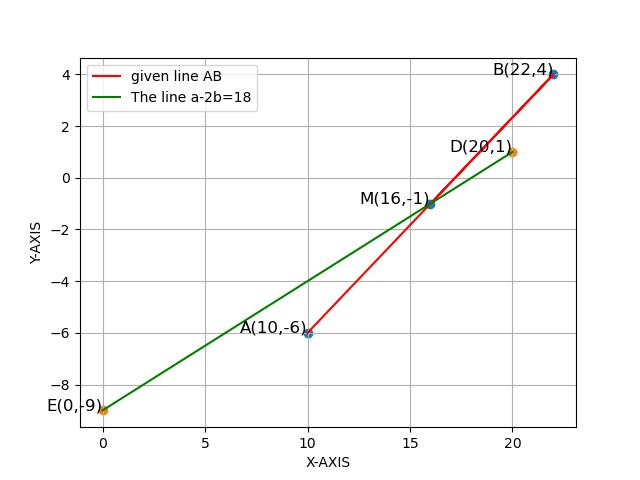
\includegraphics[width=0.7\linewidth]{figs/value.jpg}
    \caption{}
    \label{fig:enter-label}
\end{figure}
\end{frame}
\begin{frame}[fragile]
\frametitle{Functions defined}
\begin{verbatim}

#include <stdio.h>
#include <math.h>
float mp(float a, float b )
{
	return (a+b)*0.5 ;
}

float norm(float a, float b, float c, float d )
{
    return sqrt(pow(a-c,2) + pow(b-d,2)) ;
}

\end{verbatim}
\end{frame}
\begin{frame}[fragile]
\frametitle{C-Code}
\begin{verbatim}
    int main(void)
{
	FILE *ptr; 
	ptr=fopen("main.txt", "w");
	float mp(float, float) ;
	float norm(float, float, float, float) ;
	float midp1, midp2, dist ;
	midp1 = (float) mp(10,22);
	midp2 = (float) mp(-6,4);
	dist = (float) norm(10,-6,22,4);
        fprintf(ptr, "%f\n", midp1 );
	fprintf(ptr, "%f\n", midp2 );
	fprintf(ptr, "%f", dist );
        fclose(ptr) ;
	return 0;
}
\end{verbatim}
\end{frame}

\begin{frame}[fragile]
  \frametitle{Python Code }

\begin{lstlisting}[language=Python]
from ctypes import*
import matplotlib.pyplot as plt
import numpy as np
rel = CDLL('./func.so')
a = 10
b = -6
c = 22
d = 4
mp = rel.mp
mp.restype = c_float
norm = rel.norm
norm.restype = c_float
filename = 'main.txt'
with open(filename,'r') as file:
    data = file.readlines()
    print (data)


\end{lstlisting}
\end{frame}
\begin{frame}[fragile]
  \frametitle{Python Code }

\begin{lstlisting}[language=Python]
dist = norm(c_float(a), c_float(b), c_float(c), c_float(d)) 
print(dist)

x = [10, 22, mp(c_float(a), c_float(c)) ]
y = [-6, 4, mp(c_float(b), c_float(d)) ]
label = ['A(10,-6)', 'B(22,4)', 'M(16,-1)']
plt.scatter(x,y)
plt.text(x[0], y[0], label[0], fontsize=12, ha='right')
plt.text(x[1], y[1], label[1], fontsize=12, ha='right')
plt.text(x[2], y[2], label[2], fontsize=12, ha='right')
w = [20, 0] 
z = [1, -9]
labell = ['D(20,1)', 'E(0,-9)']
plt.scatter(w,z)
plt.text(w[0], z[0], labell[0], fontsize=12, ha='right')
plt.text(w[1], z[1], labell[1], fontsize=12, ha='right')

\end{lstlisting}
\end{frame}

\begin{frame}[fragile]
\frametitle{Python Code}

\begin{lstlisting}[language=Python]

plt.plot (x,y,color='red', linestyle='-', label='given line AB')
plt.plot (w,z,color='green', linestyle='-', label='The line a-2b=18')
plt.xlabel('X-AXIS')
plt.ylabel('Y-AXIS')
plt.grid()
plt.legend()
plt.show()
\end{lstlisting}
\end{frame}
\end{document}
